\documentclass[10pt]{article}\usepackage[]{graphicx}\usepackage[]{color}
%% maxwidth is the original width if it is less than linewidth
%% otherwise use linewidth (to make sure the graphics do not exceed the margin)
\makeatletter
\def\maxwidth{ %
  \ifdim\Gin@nat@width>\linewidth
    \linewidth
  \else
    \Gin@nat@width
  \fi
}
\makeatother

\definecolor{fgcolor}{rgb}{0.345, 0.345, 0.345}
\newcommand{\hlnum}[1]{\textcolor[rgb]{0.686,0.059,0.569}{#1}}%
\newcommand{\hlstr}[1]{\textcolor[rgb]{0.192,0.494,0.8}{#1}}%
\newcommand{\hlcom}[1]{\textcolor[rgb]{0.678,0.584,0.686}{\textit{#1}}}%
\newcommand{\hlopt}[1]{\textcolor[rgb]{0,0,0}{#1}}%
\newcommand{\hlstd}[1]{\textcolor[rgb]{0.345,0.345,0.345}{#1}}%
\newcommand{\hlkwa}[1]{\textcolor[rgb]{0.161,0.373,0.58}{\textbf{#1}}}%
\newcommand{\hlkwb}[1]{\textcolor[rgb]{0.69,0.353,0.396}{#1}}%
\newcommand{\hlkwc}[1]{\textcolor[rgb]{0.333,0.667,0.333}{#1}}%
\newcommand{\hlkwd}[1]{\textcolor[rgb]{0.737,0.353,0.396}{\textbf{#1}}}%
\let\hlipl\hlkwb

\usepackage{framed}
\makeatletter
\newenvironment{kframe}{%
 \def\at@end@of@kframe{}%
 \ifinner\ifhmode%
  \def\at@end@of@kframe{\end{minipage}}%
  \begin{minipage}{\columnwidth}%
 \fi\fi%
 \def\FrameCommand##1{\hskip\@totalleftmargin \hskip-\fboxsep
 \colorbox{shadecolor}{##1}\hskip-\fboxsep
     % There is no \\@totalrightmargin, so:
     \hskip-\linewidth \hskip-\@totalleftmargin \hskip\columnwidth}%
 \MakeFramed {\advance\hsize-\width
   \@totalleftmargin\z@ \linewidth\hsize
   \@setminipage}}%
 {\par\unskip\endMakeFramed%
 \at@end@of@kframe}
\makeatother

\definecolor{shadecolor}{rgb}{.97, .97, .97}
\definecolor{messagecolor}{rgb}{0, 0, 0}
\definecolor{warningcolor}{rgb}{1, 0, 1}
\definecolor{errorcolor}{rgb}{1, 0, 0}
\newenvironment{knitrout}{}{} % an empty environment to be redefined in TeX

\usepackage{alltt}

\usepackage{amsmath,amssymb,amsthm}
\usepackage{fancyhdr,url,hyperref}
\usepackage{graphicx,xspace}
\usepackage{tikz}
\usetikzlibrary{shapes,arrows,decorations.pathmorphing,backgrounds,positioning,fit,through}

\oddsidemargin 0in  %0.5in
\topmargin     0in
\leftmargin    0in
\rightmargin   0in
\textheight    9in
\textwidth     6in %6in
%\headheight    0in
%\headsep       0in
%\footskip      0.5in

\newtheorem{thm}{Theorem}
\newtheorem{cor}[thm]{Corollary}
\newtheorem{obs}{Observation}
\newtheorem{lemma}{Lemma}
\newtheorem{claim}{Claim}
\newtheorem{definition}{Definition}
\newtheorem{question}{Question}
\newtheorem{answer}{Answer}
\newtheorem{problem}{Problem}
\newtheorem{solution}{Solution}
\newtheorem{conjecture}{Conjecture}

\pagestyle{fancy}

\lhead{\textsc{Prof. McNamara}}
\chead{\textsc{SDS/MTH 291: Lecture notes}}
\lfoot{}
\cfoot{}
%\cfoot{\thepage}
\rfoot{}
\renewcommand{\headrulewidth}{0.2pt}
\renewcommand{\footrulewidth}{0.0pt}

\newcommand{\ans}{\vspace{0.25in}}
\newcommand{\R}{{\sf R}\xspace}
\newcommand{\cmd}[1]{\texttt{#1}}
\DeclareMathOperator{\Ex}{\mathbb{E}}
\DeclareMathOperator{\Var}{\text{Var}}
\DeclareMathOperator{\X}{\mathbf{X}}
\DeclareMathOperator{\Hatmat}{\mathbf{H}}

\rhead{\textsc{December 6, 2016}}
\IfFileExists{upquote.sty}{\usepackage{upquote}}{}
\begin{document}

\paragraph{Agenda}
\begin{enumerate}
  \itemsep0em
  \item Presentations and final reports
  \item A little more logistic regression
  \item Putting it all together
\end{enumerate}



\paragraph{Project} 
Some important things to keep in mind:
\begin{itemize}
\item For the presentation, you will only have 8 minutes. Going over time is a surefire way to lose points. Going under time is fine.
\item Please focus your presentation only on one model (your current favorite). You should convince us the problem is interesting, interpret the coefficients in the context of the problem, and (briefly!) show us the conditions for regression. 
\item We'll spend some time next week talking about ways to make your final project report look pretty, but remembering \verb#message=FALSE# is a big one. 
\end{itemize}

\paragraph{Coefficient interpretation} Because interpreting coefficients is so important for both your project and your test, lets practice writing out the ``script'' for a variety of cases. 

\begin{enumerate}
\itemsep0.5in
\item Multiple regression: categorical variable
\item Multiple regression: numeric variable
\item Multiple regression: interaction term
\item ANOVA $\alpha_i$
\item ANOVA $\mu_i$
\item Logistic regression: categorical variable
\item Logistic regression: numeric variable
\item Logistic regression: interaction term
\end{enumerate}

\paragraph{Logistic regression}
Let's pull the example of med school acceptance through the three `spaces' for logistic regression to see how it applies.



\begin{knitrout}\footnotesize
\definecolor{shadecolor}{rgb}{0.969, 0.969, 0.969}\color{fgcolor}\begin{kframe}
\begin{verbatim}
##           Sex
## Acceptance  F  M
##          0 10 15
##          1 18 12
\end{verbatim}
\end{kframe}
\end{knitrout}


\paragraph{Probability}
	\begin{eqnarray*}
			\pi &=& \frac{e^{\beta_0 + \beta_1\cdot X}}{1 + e^{\beta_0 + \beta_1\cdot X}}
		\end{eqnarray*}
		The probability form is how the model gets fit, but it does not have an easy interpretation for what happens with a change in $x$. 
		
\begin{knitrout}\footnotesize
\definecolor{shadecolor}{rgb}{0.969, 0.969, 0.969}\color{fgcolor}
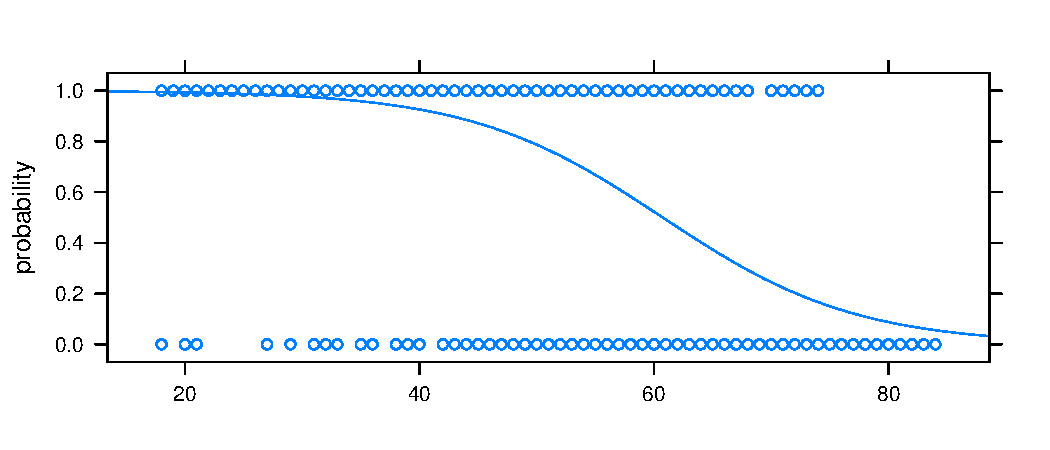
\includegraphics[width=\maxwidth]{figure/unnamed-chunk-4-1} 

\end{knitrout}

What is the probability of getting into med school for a woman? For a man? 
\vspace{0.5in}
\paragraph{Odds}
		
		\begin{eqnarray*}
	    \frac{\pi}{1-\pi} &=& e^{\beta_0 + \beta_1\cdot X}
		\end{eqnarray*}

Odds are useful when you want to interpret the slope coefficient. We can use the interpretation, ``A one unit increase in $x$ is associated with changing the odds by a factor of $e^{\beta_1}$. 

\begin{knitrout}\footnotesize
\definecolor{shadecolor}{rgb}{0.969, 0.969, 0.969}\color{fgcolor}
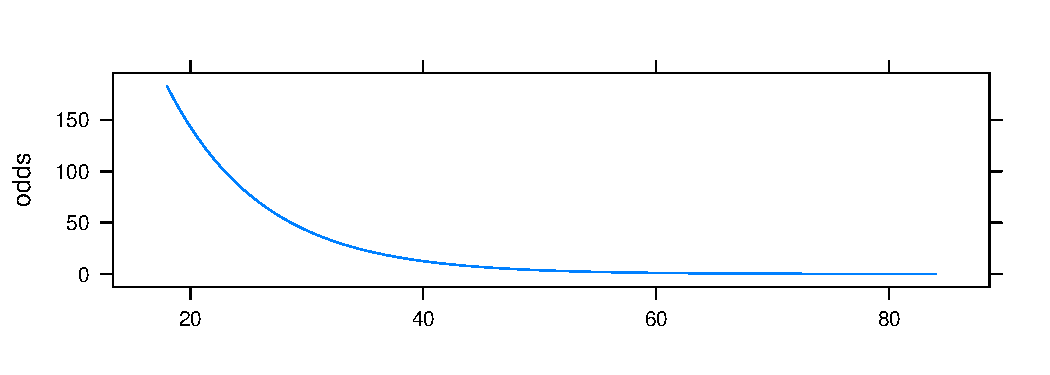
\includegraphics[width=\maxwidth]{figure/unnamed-chunk-5-1} 

\end{knitrout}

What are the odds of getting into med school for a woman? For a man? What is the odds ratio?
\vspace{0.5in}
\paragraph{Log odds}
	\begin{eqnarray*}
			\log \left( \frac{\pi}{1-\pi} \right) &=& \beta_0 + \beta_1\cdot X \\
		\end{eqnarray*}
		
		Thinking about log odds is useful when you want a linear form of a regression line. You can interpret the coefficients in the standard way we have been doing for linear regression, ``A one unit increase in $x$ is associated with a $\beta_1$ increase in the log odds of $y$''
		
\begin{knitrout}\footnotesize
\definecolor{shadecolor}{rgb}{0.969, 0.969, 0.969}\color{fgcolor}
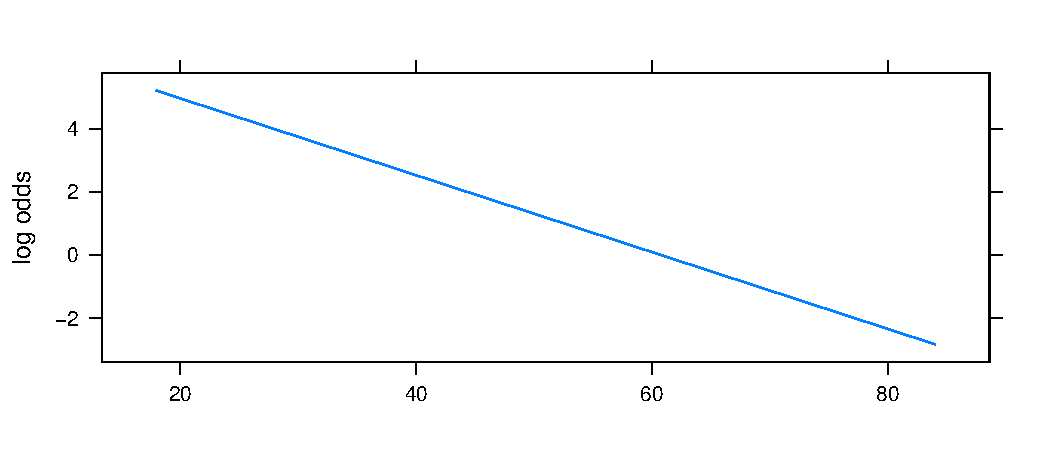
\includegraphics[width=\maxwidth]{figure/unnamed-chunk-6-1} 

\end{knitrout}
	
What is the empirical logit for getting into med school for a woman? For a man? 
\vspace{0.5in}
\begin{knitrout}\footnotesize
\definecolor{shadecolor}{rgb}{0.969, 0.969, 0.969}\color{fgcolor}\begin{kframe}
\begin{verbatim}
## 
## Call:
## glm(formula = Acceptance ~ Sex, family = binomial, data = MedGPA)
## 
## Deviance Residuals: 
##    Min      1Q  Median      3Q     Max  
## -1.435  -1.084   0.940   0.940   1.274  
## 
## Coefficients:
##             Estimate Std. Error z value Pr(>|z|)
## (Intercept)   0.5878     0.3944   1.490    0.136
## SexM         -0.8109     0.5528  -1.467    0.142
## 
## (Dispersion parameter for binomial family taken to be 1)
## 
##     Null deviance: 75.791  on 54  degrees of freedom
## Residual deviance: 73.594  on 53  degrees of freedom
## AIC: 77.594
## 
## Number of Fisher Scoring iterations: 4
\end{verbatim}
\end{kframe}
\end{knitrout}
\clearpage
Write out the equation for the model in each of the three formats. 
\vspace{2in}

How do you interpret the coefficient on \verb#SexM#?
\vspace{0.5in}

\paragraph{Putting it all together}
Lets consider the material we have covered throughout this course. We have tried to focus mostly on applied ideas, some of which are computational (more useful in practice, hard to test) and some which are slightly more theoretical (needed so you understand what you can apply, easier to test).

Lets try to categorize some of the tasks we have learned how to perform. Where in the CFAU process do these fit?
\\ Interpreting multiple regression coefficients, nested F-tests, added variable plots, stepwise regression, calculating Cook's distance, calculating Fisher's LSD, calculating Tukey's HSD, the Bonferroni correction, randomization tests, bootstrap methods, fitting ANOVA, rewriting ANOVA models in different ways, checking ANOVA p-values, fitting a logistic regression model, translating from log-odds to odds, translating from odds to probability, calculating odds ratios, looking at p-values on logistic regression, interpreting logistic regression coefficients, considering forms of models. 
\\
Choose
\vspace{1in}
\\
Fit
\vspace{1in}
\\
Assess
\vspace{1in}
\\
Use
\vspace{1in}



\end{document}
